\documentclass[11pt,a4paper,leqno]{article}
\usepackage{a4wide}
\usepackage[T1]{fontenc}
\usepackage[utf8x]{inputenc}
\usepackage{lmodern,textcomp}
\usepackage{float, afterpage, rotating, graphicx}
\usepackage{longtable, booktabs, tabularx}
\usepackage{verbatim}
\usepackage{eurosym, calc, chngcntr}
\usepackage{amsmath, amssymb, amsfonts, amsthm, bm, delarray} 
\usepackage{caption}
\usepackage{datetime}
\usepackage{tkz-graph}
\usepackage{enumitem}
\usepackage[multiple]{footmisc}
\usepackage{multirow}
\usepackage{pdfpages}
\usetikzlibrary{arrows,positioning,snakes,shapes,shapes.multipart,patterns,mindmap,shadows}
\usepackage{natbib}
\usepackage{subcaption}
\bibliographystyle{chicago}


\usepackage[tikz]{bclogo}

\usepackage[framemethod=tikz]{mdframed}
\mdfdefinestyle{mystyle}{%
	rightline=true,
	innerleftmargin=10,
	innerrightmargin=10,
	outerlinewidth=3pt,
	topline=false,
	rightline=true,
	bottomline=false,
	skipabove=\topsep,
	skipbelow=\topsep
}

\begin{document}
 \begin{center}
	\begin{LARGE}
		\textbf{
			ASP Course on Microeconometric Methods (2021)\\
			 - Take Home Assignment -\\
		}
	\end{LARGE}
	\vspace{0.2cm}
	{\large \textbf{Project A}} \\\vspace{0.2cm}
	{\large \textbf{Susann Adloff, Linda Maokomatanda, Saskia Meuchelböck}} \vspace{0.2cm}
\end{center}

\section*{Section 1}
We review three papers that provide a seamless synergy into our project that estimates the impact of foreign direct investment on firm performance by taking a holistic approach to the literature. We first take a look at a paper by \cite{borin2016foreign} which displays the effects on firm performance in the firm’s country of origin when they decide to invest abroad, thus becoming a multi-national enterprise. In an intermediate stage, we review a paper by Bajgar and Javorcik (2020)  that investigates analyze spillover effects from FDI on domestic firm performance resulting from links along the supply chain. To conclude our review and introduce section 2, we review \cite{chen2011} studies the role of the origin of FDIs on target firm performance changes.

\cite{borin2016foreign} investigate the ex-post effects of foreign direct investment (FDI) on firm performance using data from the Bank of Italy’s annual Survey of Industrial and Service Firms (the Invind survey) as well as balance sheet data from the Company Accounts Data Service (henceforth CADS).  They extend the discussion from empirical and theoretical literature that shows how multinational firms (MNE) exhibit a competitive advantage before investing abroad, by conducting microeconomic data analysis to evaluate the policy implications of firm heterogeneity. The authors specify the best-case scenario to be the implementation of policy measures and internationalization strategies that are capable of enhancing both firm performance and employment. The ex-ante causal relationship (from performance to internationalization) in \cite{borin2016foreign}’s paper introduces a severe form of endogeneity, in that ex-post performance might reflect not only foreign investment, but also pre-existent advantages in terms of managerial ability, know-how and technology. To accurately evaluate the ex-post effects of FDI that take into account the inherent self-selection problem, the authors use a propensity score matching procedure to analyze the causal relationship between firm performance and foreign direct investment, looking in particular at the potential gains in terms of productivity and potential losses in terms of employment in the parent firm due to the acquisition of multinational status; as well as to evaluate whether these effects are evenly spread across new MNEs or concentrated among certain groups of investors. To implement the propensity matching estimation, the authors choose a company, ex-ante very similar to the first one, but that does not choose to invest abroad to act as a proxy of the unobservable counterfactual, enabling them to compare the evolution of new MNEs with the performance of the exact same company with no investment; since it is not possible to observe the same company in these two different scenarios. They find that firms investing abroad for the very first time, especially in advanced economies, show higher productivity and employment dynamics in the years following the investment: the average positive effect on TFP is driven by new multinationals operating in specialized and high-tech sectors, while the positive employment gains are explained by an increase of the white collar component. On average, the authors do not find a negative effects on the parent firm's blue collar component.

\cite{bajgar2020climbing} analyze spillover effects from FDI on domestic firm performance resulting from links along the supply chain. More specifically, they investigate the relationship between quality upgrading by Romanian exporters and the presence of foreign affiliates in upstream and downstream industries, respectively. They use customs data merged with firm-level data for the years 2005 to 2011 and find a positive and robust link between the product quality of domestic exporters – proxied by two measures established in the literature, namely unit values and a measure proposed by \cite{khandelwal2013trade} – and the presence of foreign-owned firms in upstream (i.e. input-supplying) industries. The results indicate that a one percentage point increase in FDI presence upstream is related to a roughly 0.5\% increase in product quality of domestic exporters, on average and ceteris paribus. The positive relationship between export quality and the presence of foreign-owned firms in downstream industries is less robust. To estimate these effects, the authors employ OLS regressions with product quality as the dependent variable and a measure of FDI presence in upstream and downstream industries, respectively, as the main independent variable of interest. They control for firm-product-destination fixed effects, region-time fixed effects and linear time trends at the region-industry level. However, the authors acknowledge that reverse causality could be a problem, for example if foreign firms primarily invest in industries where high-quality domestic inputs become increasingly available, and these developments are not captured by the linear time trends. To mitigate these concerns, they lag their FDI variables by one year in all specifications. In addition, they perform a “strict exogeneity” test suggested by \cite{wooldridge2010econometric}, including also contemporaneous and lead FDI values into their model. They argue that if foreign firms enter Romania as a consequence of quality upgrading rather than the other way around, the coefficients on the lead values of FDI should also be statistically significant, which is not the case. They conclude that the increase in foreign presence in the upstream industries over the studied period corresponded to a circa 4\% increase in the quality of exports by local firms.

\cite{chen2011} studies the role of the origin of FDIs on target firm performance changes. It uses data on acquisitions of U.S firms between 1979 and 2006, comparing firm level performance indicators before and after acquisition, focusing on the difference between firms acquired by domestic firms (USFs), firms from industrialized countries (ICFs) and firms from developing countries (DCFs). The identification strategy is based on a diff-in-diff analysis which gives rise to a twofold selection problem. The empirical set up defines a control group which is domestically acquired firms and two treatment groups. As trans-boundary firm acquisition is more challenging than domestic acquisitions (Helpman et al 2004), firms that engage in the former are likely to be different from those that invest domestically, which might translate into "more skillful" target firm selection on part of foreign acquirers. Hence, the firms chosen for foreign investments are likely to structurally differ pre-treatment from those firms that are chosen for domestic acquisitions. Secondly, selection criteria for target firms might also differ based on the origin of the acquiring firm. The author argues that systematic differences can be expected in the aimed at restructuring process depending on the origin of the acquirer, due to structural differences between these groups in technological progress and relative input costs between target and acquirer. Consequently, selection bias might be found in the comparison of control and the treatment groups, as well as in the comparison of the two treatment groups. To solve this issue the author implements a propensity score matching procedure. The scoring is achieved through a multinomial logit model estimation of observables available to acquires before the acquisition that provide information on present and potential future target firm performance, as well as year, industry and state fixed effects. The matching is done using a kernel matching procedure. This step allows to impose pre-treatment homogeneity in firm performance across comparison groups and thus to interpret any difference in performance between matched pairs to result from the difference in treatment. The results of this estimation show that firms acquired by ICFs show 13\% higher improvements in terms of labour productivity, a 10\% higher profit increase and a 19\% higher increase in sales in the five years post acquisition relative to the year before the acquisition, compared to firms acquired by USFs. Between those two groups no difference in overall employment changes was found. For firms acquired by DCFs the author finds that labour productivity gains and changes in sales and employment are 1\% lower than those of domestic acquisitions, albeit higher profit gains. Comparing firm-level effects of FDIs originating from industrialized countries to those from developing countries, gains in sales, labour productivity and employment are significantly higher for target firms acquired by ICFs.

In Section $2$, we will provide a discussion of the most important features of the data we will be working with, including some interesting patterns and correlations that we have discovered in the data. We also provide some summary statistics and graphs of the variables of interest.

\section*{Section 2} (Saskia)
\textit{Provide a discussion of the most important features of the data; describe any interesting patterns or correlations in the data and provide some summary statistics/graphs of the variables of interest. If you have performed any data cleaning exercises (e.g. you have excluded some observations) or carried out any data transformations (e.g. “unlogging” the wage variables).}

\begin{itemize}
	\item full sample description:
	\begin{itemize}
		\item dataset on firm level performance indicators for the years 2015 and 2017 for 11.323 firms  
		\item roughly one third each low tech and medium high tech industries, and one sixth each medium low tech and high tech industries
		\item 40\% independent firms, 30\% state owned firms, roughly 20\% subsidiaries and a minority of 8\% listed companies.  
	\end{itemize}
	\item treatment var: FDI received in 2016 yes or no and which type of FDI
	\begin{itemize}
		\item 39\% of firms in the dataset did receive FDIs
		\item 8\% of all firms in the dataset received export oriented FDIs, 14\% technology intensive FDIs and 17\% domestic market seeking ones
	\end{itemize}

		%\textit{interesting patterns or correlations?!?!?}
\end{itemize}

\section*{Section 3} (Susann)
\textit{Explain very briefly your econometric approach to evaluate the casual effects of FDI on the outcome variables of choice (you can assume that the readers know the basic principles of propensity score-based estimators). You are encouraged to estimate more than one model and probe the sensitivity of your findings to alternative model specifications. Write a report on your main findings, indicating which of the estimators, if any, you would you prefer most in the context of this exercise, and why?}

The challenge that this dataset poses for the identification of causal effects of FDI, is that the treatment (FDI) is not assigned randomly across firms but the result of a selection process. Investors will carefully decide which firms to invest in using observable firm-level performance indicators before investing. Thus, treatment allocation will likely depend on observable firm characteristics in 2015, such that firms in the treatment group will structurally differ from firms in the untreated group. Table \ref{balance_check} shows that in the available dataset this imbalance in pre-treatment characteristics between treated and non-treated firms can be found across all available performance indicators from 2015. In addition, table \ref{selection_logit} presents the result of a logit regression of FDI on pre-treatment characteristics, which corroborates the statistical significance of correlations with FDI assignment for all available pre-treatment variables expect log wages. The set of pre-treatment firm characteristics is, consequently, correlated with post-treatment performance as well as with treatment allocation, which violates the conditional independence assumption, necessary for causal identification. As this violation is found across multiple variables, the data suffers from what is called \textit{the curse of dimensionality}. This can be circumvented by propensity score matching such that causal identification of FDI effects on firm performance can still be achieved. In particular, we will investigate the impact of FDIs on firm employment and wages.\\ \par 

 \begin{table}[htbp]\centering
\def\sym#1{\ifmmode^{#1}\else\(^{#1}\)\fi}
\caption{Logit estimation results of FDI on pre-treatment observables \label{selection\_logit}}
\begin{tabular}{l*{1}{cc}}
\hline\hline
                &\multicolumn{2}{c}{(1)}\\
                &\multicolumn{2}{c}{FDI/TREATMENT dummy in 2016}\\
                &        b   &       se\\
\hline
FDI/TREATMENT dummy in 2016&            &         \\
Wages in 2015 (logs)&  -0.0008   &  (0.008)\\
Total factor productivity in 2015&  -0.0917***&  (0.016)\\
Employment in 2015 (logs)&   0.1905***&  (0.011)\\
Export intensity in 2015&  47.2347***&  (0.765)\\
Debt in 2015 (logs)&  -0.3426***&  (0.109)\\
RD in 2015 (dummy)=0&   0.0000   &      (.)\\
RD in 2015 (dummy)=1&   0.2892***&  (0.097)\\
Low-tech        &   0.0000   &      (.)\\
Medium low      &  -2.1258***&  (0.104)\\
Medium high     &  -5.0274***&  (0.112)\\
High-tech       &  -8.5163***&  (0.164)\\
 Listed companies&   0.0000   &      (.)\\
 Subsidiaries   &   1.8301***&  (0.148)\\
 Independent    &   3.4707***&  (0.150)\\
 State          &   2.1772***&  (0.151)\\
No ports within 500km&   0.0000   &      (.)\\
Ports within 500km&  -3.0085***&  (0.087)\\
Constant        &  -7.0707***&  (0.212)\\
\hline
Observations    &    11323   &         \\
\hline\hline
\end{tabular}
\end{table}



% check balancedness computationally, check significance of all variables
 
 In order for propensity score matching to successfully alleviate any concerns of selection bias, a scoring function needs to be identified that achieves balancedness in terms of relevant observables, on one hand, and a good common support, i.e. overlap on the other. This is not trivial. Imagine a situation in which treatment is assigned according to one specific set of variables. Whenever values of this set of variables are high a subject receives treatment. If scoring is performed based on this variable set then propensity scores will be high for firms with high values along this set of variables and matching of firms with similar propensity scores will produce very little differences in values of these variables. Yet, this will produce a most certainly bad overlap. Opposed to that using a variable that is not related to treatment assignment for the propensity score matching will produce a high overlap as propensity scores calculated based on a unrelated variable will be similarly distributed within treatment and non-treatment groups, but it will be unlikely that this matching procedure will be able to balance the previously unbalanced variables. Consequently, a scoring function specification has to be found that balances all variables relevant for treatment assignment but in a way that produces high overlap. \\ \par 
 
 In the dataset at hand all pre-treatment performance indicators showed relevance for selection, except for log wages, which however exhibits pre-treatment imbalance between groups. Figure \ref{ol_linlog1} shows the overlap and table \ref{bal_linlog1} the balancedness check results of a linear functional specification including all these variables in a logit scoring function. It can be seen that this functional specification is not suited to achieve sample balance in a 1 on 1 matching procedure and most importantly not providing sufficient overlap to identify an unbiased average treatment effect. Varying the functional specification in multiple ways (using probit instead of logit, interacting continuous performance indicators with categorical type determinants) does not produce any considerable improvements in overlap (compare figure \ref{ol_intlog1} and \ref{ol_intprob1} in the Appendix). If we reduce the number of variables used in the scoring function to a subset of the pre-treatment observables, we find improvements in overlap as is expected based on the above presented argument (compare e.g. figure \ref{ol_linlog1_red}). However, this comes at the cost of missing control over several variables that could be shown to significantly drive selection. In an attempt to reduce dimensionality of the information used in the scoring function while keeping control over all variables relevant for selection we opt for translating continuous performance indicators into less fine grained categorical variables. In particular, we construct a variable "EXP2015\_CAT" that assigns the values 0, 1 or 2 for firms that have an export intensity of 0, below 25\% or larger 25\% respectively. Using a scoring function in which the remaining continuous variables are interacted with the binary/ categorical variables including "EXP2015\_CAT" achieves strong improvements in overlap compared to the other specifications based on the full set of variables (see figure \ref{ol_intcatlog1}). In addition, we find acceptable balancedness levels in the one on one matching, with matched differences of close to or above 0.2 in only two cases (compare table 2). Testing various alternative matching specifications such as matching with the two or four nearest neighbours or using a caliper (compare tables \ref{bal_intcatlog2} and \ref{bal_intcatlog4} in the Appendix) shows that the best results seem indeed to be achieved in a one on one matching. Given this turnout, this specification is chosen for effects estimation.\\ \par

\begin{table}
	\centering
\begin{tabular}{lcccc}
	                    &    r(table)&            &            &            \\
                    &    Diff:Raw&  Diff:Match&   Ratio:Raw& Ratio:Match\\
log wages in 2015   &   -.1300321&   -.0515036&    .9769191&    .8845742\\
Total factor productivity in 2015&    -.178877&    .2139231&    .9473458&    .4003003\\
log of employment in 2015&    .5654306&    -.156559&     .803081&    .6229867\\
EXPORT INTENSITY in 2015&    1.014184&    .5934387&    1.228659&    1.336483\\
 log of DEBTS in 2015&   -.0529435&   -.2515877&    1.051101&    1.021671\\
R\&D dummy in 2015=1&    .0356507&   -.0076941&    1.085768&    .9795245\\
Medium low-tech industries&    .1206088&   -.0152956&    1.263082&    .9634731\\
Medium high-tech industries&   -.2329159&   -.1939862&    .8156583&    .7717778\\
High-tech industries&   -.5425507&    .4301909&    .2855456&    1.693899\\
 Subsidiaries       &    -.018354&    -.088095&    .9769702&     .858366\\
 Independent        &    .0616272&   -.0365731&     1.02321&    .9742405\\
 State              &    .1016402&   -.4001546&    1.100951&    .7088027\\
Ports within 500km  &    .4092869&   -.3412843&    1.253595&    .8230184\\

\end{tabular}
	\caption{Balance check: linear logit 1 on 1}
	\label{bal_linlog1}
\end{table}

\begin{figure}
	\centering
	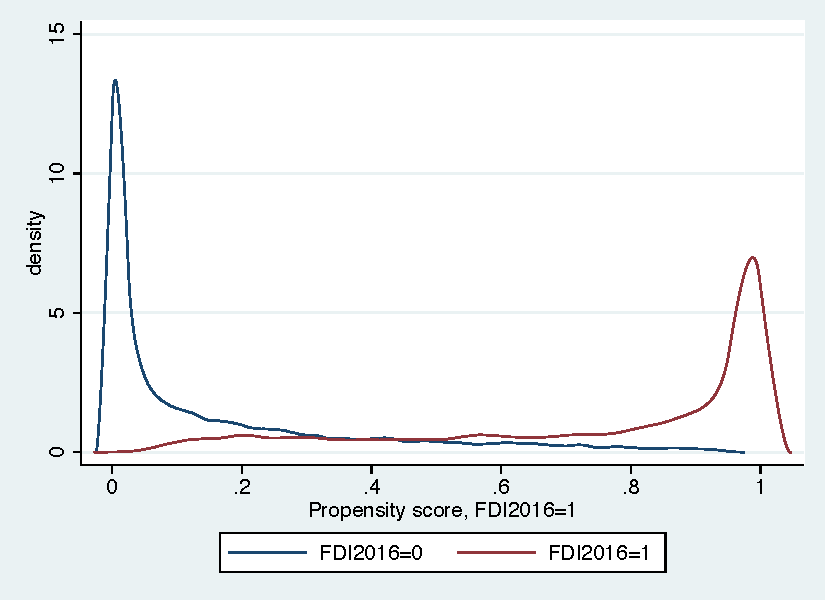
\includegraphics[scale=0.6]{figures_and_tables/3_overlap_linearlogit1o1.pdf}\
	\caption{Overlap: linear logit 1 on 1 }
	\label{ol_linlog1}
\end{figure}

\begin{figure}
	\centering
	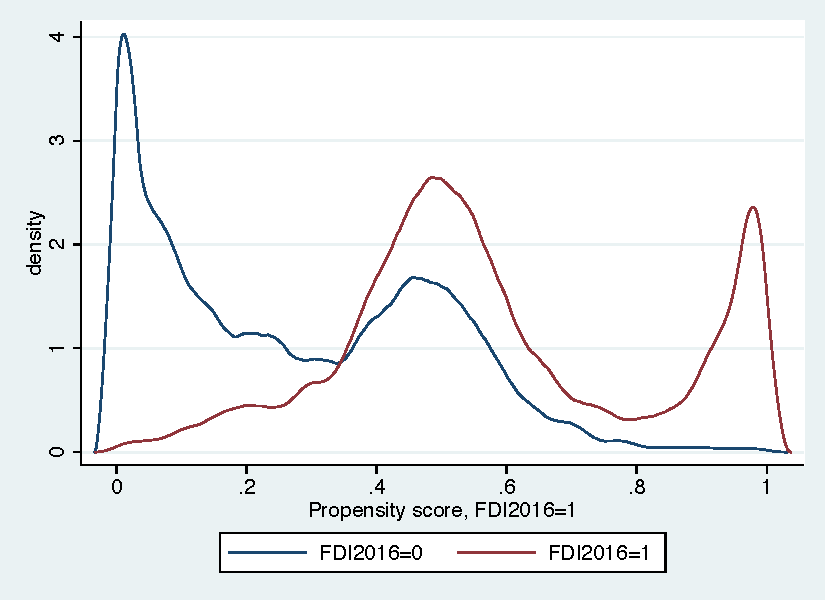
\includegraphics[scale=0.6]{figures_and_tables/3_overlap_intcatlogit1o1.pdf}\
	\caption{Overlap: interactions using exports as categorical instead of continuous variable logit 1 on 1 }
	\label{ol_intcatlog1}
\end{figure}

\begin{table}
	\centering
	\begin{tabular}{lcccc}
	 
            &    Diff:Raw&  Diff:Match&   Ratio:Raw& Ratio:Match\\ \hline
0b.RD2015xc.logwages2015&   -.1195646&    .0525046&     .947075&    1.062749\\
1.RD2015xc.logwages2015&    .0055913&    .0576109&    .9912599&    1.274914\\
1b.TECHxc.logwages2015&    .4099088&    .0288036&    1.446385&    1.012937\\
2.TECHxc.logwages2015&    .0985765&    .0376167&    1.221177&    1.078534\\
3.TECHxc.logwages2015&   -.1947846&   -.0195882&    .7998561&    1.077204\\
1b.OWNxc.logwages2015&   -.2416651&   -.0406993&    .3646025&    .8427318\\
2.OWNxc.logwages2015&   -.0501523&    -.078579&    .8787442&    .8758421\\
3.OWNxc.logwages2015&    .0095374&    .0352781&    .9615021&    1.109249\\
0b.PORTxc.logwages2015&   -.3780525&    .1273289&    .9245549&    1.141669\\
1b.EXP2015\_CATxc.logwages2015&   -.4723787&    .0947225&    1.179189&    1.081208\\
0b.RD2015xc.TFP2015&   -.1739665&   -.0203347&    .9100893&    .9091296\\
1.RD2015xc.TFP2015&    .0080044&    .0443347&    .9791256&    1.135322\\
1b.TECHxc.TFP2015&    .3830039&    .0387406&    1.517568&     1.02464\\
2.TECHxc.TFP2015&    .0592069&    .0218559&     1.09476&    1.039168\\
3.TECHxc.TFP2015&   -.2626395&   -.0332445&    .6142341&    .9655526\\
1b.OWNxc.TFP2015&   -.2670312&   -.0571476&    .2665297&     .720536\\
2.OWNxc.TFP2015&    -.064156&   -.0762223&    .8276227&    .8391969\\
3.OWNxc.TFP2015&   -.0408866&    .0100326&    .8831729&    .9812749\\
0b.PORTxc.TFP2015&   -.4416219&    .0380993&    .7259598&      .88749\\
1b.EXP2015\_CATxc.TFP2015&   -.4566127&    .0065822&    .9833249&    .8881018\\
0b.RD2015xc.logemp2015&    .4513985&    .1104609&    1.015839&    .7723211\\
1.RD2015xc.logemp2015&    .1258157&     .079598&    1.551717&    1.236144\\
1b.TECHxc.logemp2015&    .4601552&     .050231&    1.534047&    1.002554\\
2.TECHxc.logemp2015&    .2274026&    .0593328&    1.926955&    1.071029\\
3.TECHxc.logemp2015&    .0899055&   -.0276154&    1.370232&    .8064564\\
1b.OWNxc.logemp2015&   -.0820011&     .021356&    .9009638&     1.11227\\
2.OWNxc.logemp2015&    .1399032&   -.0275592&    1.482211&    .9386443\\
3.OWNxc.logemp2015&    .2656301&    .0867379&    1.407778&    1.052158\\
0b.PORTxc.logemp2015&    .1339363&    .2348676&     1.28113&    1.007255\\
1b.EXP2015\_CATxc.logemp2015&    .0840549&     .190327&    1.142787&    .8433407\\
0b.RD2015xc.DEBTS2015&   -.0687846&    .0401788&    1.018707&    .9555409\\
1.RD2015xc.DEBTS2015&    .0328123&    .0331289&    1.167688&    1.141984\\
1b.TECHxc.DEBTS2015&    .3620529&    .0212764&    1.493647&    1.006909\\
2.TECHxc.DEBTS2015&    .0875624&    .0375397&    1.216558&     1.07361\\
3.TECHxc.DEBTS2015&   -.1987245&   -.0448235&    .7404538&    .9192316\\
1b.OWNxc.DEBTS2015&   -.2451112&   -.0710123&    .3194455&    .6600723\\
2.OWNxc.DEBTS2015&   -.0444712&   -.0653756&    .8861299&    .9017093\\
3.OWNxc.DEBTS2015&   -.0148901&    .0526032&    .9654587&    1.074223\\
0b.PORTxc.DEBTS2015&   -.3147821&     .125639&    .9126556&    1.089006\\
1b.EXP2015\_CATxc.DEBTS2015&   -.3607874&    .0926031&    1.078069&    1.015868\\

	\end{tabular}
	\caption{Balance check: interactions using exports as categorical instead of continuous variable logit 1 on 1}
	\label{bal_intcatlog1}
\end{table}

 Following this estimation approach, Table \ref{ates} shows the average marginal effects of FDI on firm performance with regard to employment and wages. The effect on log employment is 0.79. This translates into an increase in employment by 120\% from FDI one year after the investment took place. The average treatment effect for log wages is 0.75. In light of the overall negative trend in wage changes from 2015 to 2017, thus, wages of firms that did receive FDIs fell by 110\% less than wages of firms that did not receive any FDI.


\begin{table}[htbp]\centering
\def\sym#1{\ifmmode^{#1}\else\(^{#1}\)\fi}
\caption{Impact of FDI on Wages and Employment \label{ates}}
\begin{tabular}{l*{2}{c}}
\hline\hline
                &\multicolumn{1}{c}{(1)}&\multicolumn{1}{c}{(2)}\\
                &\multicolumn{1}{c}{Log Employment}&\multicolumn{1}{c}{Log Wages} \\ \hline \\[-1ex]
ATE             &   0.7867***&   0.7456***\\
                &  (0.194)   &  (0.181)   \\
\hline
Observations    &    11323   &    11323   \\
\hline\hline
\multicolumn{3}{l}{\footnotesize * p<0.1, ** p<0.05, *** p<0.01}\\
\end{tabular}
\end{table}


\clearpage

\section*{Section 4} (Linda)
\textit{Try to answer the question whether your conclusions from Section 3 change if you re-estimate the casual effects of FDI by type of FDI? You are encouraged to consider alternative models to estimate the propensity scores, as well as experiment with different estimators.}


--> using the models with best balancing still show bad overlap. This means that propensity scoring is difficult to apply to this data. Doubly robust can work with misspecified scoring functions use doubly robust accept some imbalance. 

\underline{Wage Effects}
\begin{itemize}
	\item matching process will be the same as before if same variables used, thus use last condition including interaction effects
	\item ATE 0.654 (p-value 0.046)
	\item looking at figure 6 it can be seen that overall drop in wages from 2015 to 2017, which were however much lower treated firms.
\end{itemize}


\begin{itemize}
	\item effects of FDI on firm performance likely varying by FDI type as FDIs differ by the kind of restructuring goals they formulate, i.e. export or domestic market oriented, thus they are likely affect different outcome variables differently
	\item also firm selection criteria are likely to differ between FDI types, given these different restructuring goals 
	\begin{itemize}
		\item for example significant differences in RD in 2015 of firms target for export oriented, technology intensive and domestic market oriented FDIs
		\item (Types quite balanced)
	\end{itemize}
	\item redo by using multinomial logit model for propensity score matching and doubly robust propensity score estimator (task 5 of computer class 2)
	
	\underline{Employment Effects}
	\begin{itemize}
		\item try 1: logit scoring function, no interactions
		\begin{itemize}
			\item imbalances in high tech industries, exports and a bit in employment
			\item ATE 0.29/0.30 for all FDI types. how can that be?!
		\end{itemize}
		\item try 2: logit scoring function, interactions 
		\begin{itemize}
			\item --> ERROR for balancing table
			\item ATE roughly the same slightly more spread around 0.30
		\end{itemize}	 
	\end{itemize}

	\underline{Wage Effects}
	\begin{itemize}
		\item try 1: no interactions --> ATE: 0.23 for all
		\item try 2: interactions --> ATE: 0.23 more spread out
	\end{itemize}
	\item check 
\end{itemize}

\section*{Section 5} 
\textit{This is a summary and conclusion section where you should give an overall evaluation of your work including possible shortcomings.}
\begin{itemize}
	\item ate or atet? substantial amount of sample outside of overlapping area. 
	\item doubly robust or nearest neighbour matching
\end{itemize}

\nocite{chen2011}
\clearpage
\bibliography{micromeths.bib}


\appendix
\section*{Appendix}
The output from Stata and the code you used in your study.

\begin{figure}
	\centering
	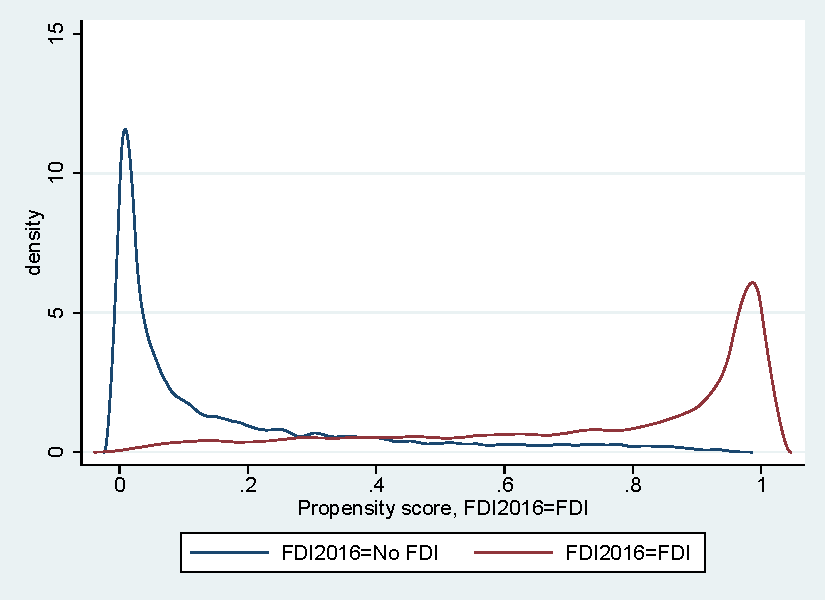
\includegraphics[scale=0.6]{figures_and_tables/3_overlap_intlogit1o1.pdf}\
	\caption{Overlap: int logit 1 on 1 }
	\label{ol_intlog1}
\end{figure}

\begin{figure}
	\centering
	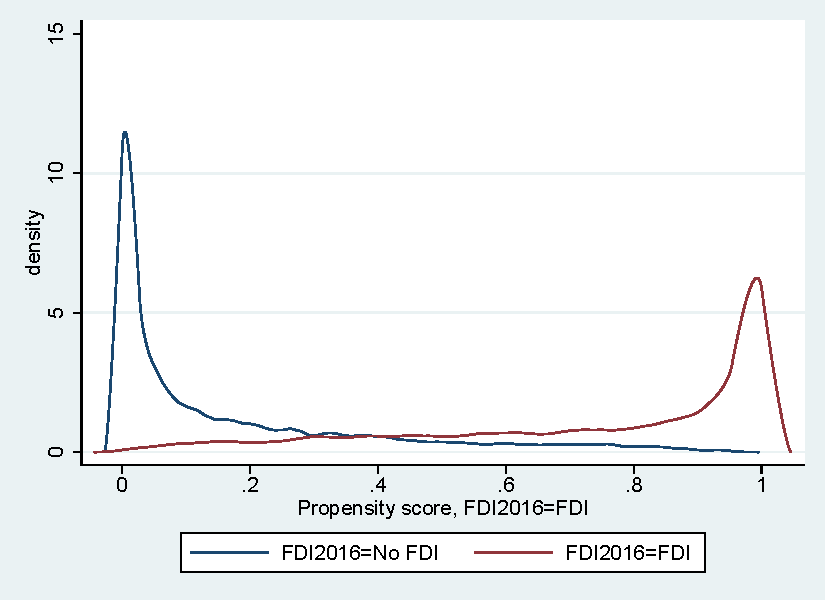
\includegraphics[scale=0.6]{figures_and_tables/3_overlap_intprobit1o1.pdf}\
	\caption{Overlap: int probit 1 on 1 }
	\label{ol_intprob1}
\end{figure}

\begin{figure}
	\centering
	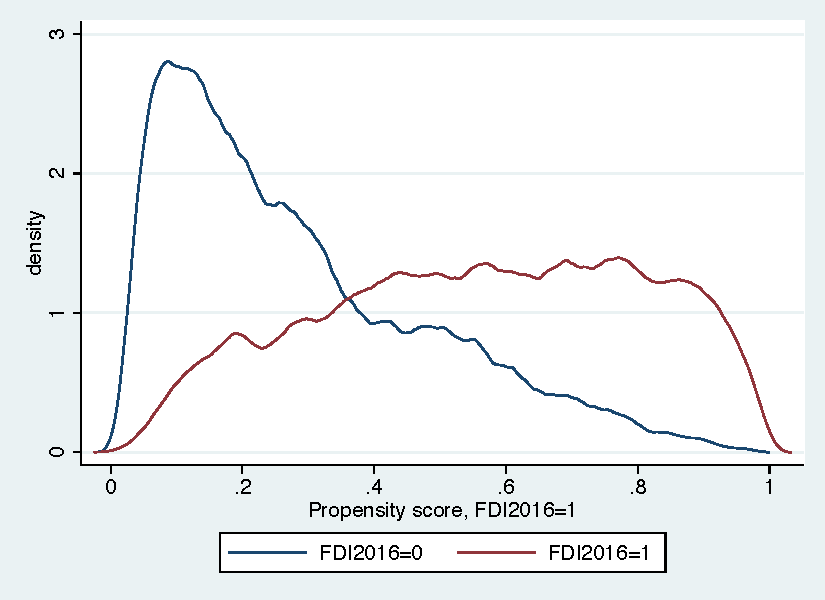
\includegraphics[scale=0.6]{figures_and_tables/3_overlap_linearlogit1o1_reduced.pdf}\
	\caption{Overlap: lin logit 1 on 1 reduced set (excl. cat/binary) }
	\label{ol_linlog1_red}
\end{figure}

\begin{table}
	\begin{tabular}{lcccc}
	            &    r(table)&            &            &            \\
            &    Diff:Raw&  Diff:Match&   Ratio:Raw& Ratio:Match\\
0b.RD2015#c.logwages2015&   -.1195646&    .0533576&     .947075&    1.083427\\
1.RD2015#c.logwages2015&    .0055913&    .0622468&    .9912599&    1.316477\\
1b.TECH#c.logwages2015&    .4099088&    .0368431&    1.446385&    1.028314\\
2.TECH#c.logwages2015&    .0985765&    .0250057&    1.221177&    1.058754\\
3.TECH#c.logwages2015&   -.1947846&   -.0206775&    .7998561&    1.052487\\
1b.OWN#c.logwages2015&   -.2416651&   -.0436965&    .3646025&     .827438\\
2.OWN#c.logwages2015&   -.0501523&    -.073387&    .8787442&    .8821358\\
3.OWN#c.logwages2015&    .0095374&    .0913069&    .9615021&    1.220857\\
0b.PORT#c.logwages2015&   -.3780525&    .1312182&    .9245549&    1.171242\\
1b.EXP2015\_CAT#c.logwages2015&   -.4723787&    .1005806&    1.179189&    1.120247\\
0b.RD2015#c.TFP2015&   -.1739665&    .0116561&    .9100893&    1.012206\\
1.RD2015#c.TFP2015&    .0080044&    .0449328&    .9791256&    1.146995\\
1b.TECH#c.TFP2015&    .3830039&    .0380806&    1.517568&    1.029373\\
2.TECH#c.TFP2015&    .0592069&    .0059181&     1.09476&    .9937183\\
3.TECH#c.TFP2015&   -.2626395&   -.0239952&    .6142341&    1.017338\\
1b.OWN#c.TFP2015&   -.2670312&   -.0545362&    .2665297&    .7563862\\
2.OWN#c.TFP2015&    -.064156&   -.0591638&    .8276227&    .8711978\\
3.OWN#c.TFP2015&   -.0408866&    .0506196&    .8831729&    1.080465\\
0b.PORT#c.TFP2015&   -.4416219&    .0664575&    .7259598&     .989018\\
1b.EXP2015\_CAT#c.TFP2015&   -.4566127&    .0384141&    .9833249&    .9922028\\
0b.RD2015#c.logemp2015&    .4513985&    .1458985&    1.015839&    .8251611\\
1.RD2015#c.logemp2015&    .1258157&    .0770499&    1.551717&    1.230311\\
1b.TECH#c.logemp2015&    .4601552&    .0557388&    1.534047&    1.003494\\
2.TECH#c.logemp2015&    .2274026&    .0438903&    1.926955&    1.024059\\
3.TECH#c.logemp2015&    .0899055&   -.0193275&    1.370232&    .8302818\\
1b.OWN#c.logemp2015&   -.0820011&    .0187964&    .9009638&    1.111048\\
2.OWN#c.logemp2015&    .1399032&   -.0080772&    1.482211&    1.009055\\
3.OWN#c.logemp2015&    .2656301&    .1355491&    1.407778&    1.151253\\
0b.PORT#c.logemp2015&    .1339363&    .2636523&     1.28113&    1.094793\\
1b.EXP2015\_CAT#c.logemp2015&    .0840549&    .2223448&    1.142787&    .9004376\\
0b.RD2015#c.DEBTS2015&   -.0687846&    .0529298&    1.018707&    .9896502\\
1.RD2015#c.DEBTS2015&    .0328123&    .0247653&    1.167688&    1.089759\\
1b.TECH#c.DEBTS2015&    .3620529&    .0286521&    1.493647&    1.017304\\
2.TECH#c.DEBTS2015&    .0875624&    .0298535&    1.216558&    1.069462\\
3.TECH#c.DEBTS2015&   -.1987245&   -.0287849&    .7404538&    .9846953\\
1b.OWN#c.DEBTS2015&   -.2451112&   -.0661205&    .3194455&    .6951376\\
2.OWN#c.DEBTS2015&   -.0444712&   -.0452431&    .8861299&    .9559771\\
3.OWN#c.DEBTS2015&   -.0148901&    .0841772&    .9654587&    1.139031\\
0b.PORT#c.DEBTS2015&   -.3147821&    .1120791&    .9126556&    1.079805\\
1b.EXP2015\_CAT#c.DEBTS2015&   -.3607874&    .0860133&    1.078069&    1.028403\\

	\end{tabular}
	\caption{Balance check: interactions using exports as categorical instead of continuous variable logit 2 on 1}
	\label{bal_intcatlog2}
\end{table}

\begin{table}
	\begin{tabular}{lcccc}
	            &    r(table)&            &            &            \\
            &    Diff:Raw&  Diff:Match&   Ratio:Raw& Ratio:Match\\
0b.RD2015#c.logwages2015&   -.1195646&    .0512606&     .947075&    1.061216\\
1.RD2015#c.logwages2015&    .0055913&    .0554608&    .9912599&    1.266693\\
1b.TECH#c.logwages2015&    .4099088&    .0453662&    1.446385&    1.037856\\
2.TECH#c.logwages2015&    .0985765&     .011763&    1.221177&    1.008307\\
3.TECH#c.logwages2015&   -.1947846&   -.0112131&    .7998561&    1.071675\\
1b.OWN#c.logwages2015&   -.2416651&     -.00517&    .3646025&    .9595119\\
2.OWN#c.logwages2015&   -.0501523&   -.0700267&    .8787442&    .8936324\\
3.OWN#c.logwages2015&    .0095374&    .0653864&    .9615021&    1.159856\\
0b.PORT#c.logwages2015&   -.3780525&     .120801&    .9245549&    1.140006\\
1b.EXP2015\_CAT#c.logwages2015&   -.4723787&    .0957885&    1.179189&    1.085749\\
0b.RD2015#c.TFP2015&   -.1739665&   -.0176556&    .9100893&    .9616481\\
1.RD2015#c.TFP2015&    .0080044&    .0449186&    .9791256&    1.144561\\
1b.TECH#c.TFP2015&    .3830039&    .0394225&    1.517568&    1.019847\\
2.TECH#c.TFP2015&    .0592069&    .0021288&     1.09476&    .9735207\\
3.TECH#c.TFP2015&   -.2626395&   -.0295988&    .6142341&    .9941437\\
1b.OWN#c.TFP2015&   -.2670312&   -.0223185&    .2665297&    .8203311\\
2.OWN#c.TFP2015&    -.064156&   -.0677646&    .8276227&    .8347698\\
3.OWN#c.TFP2015&   -.0408866&    .0193216&    .8831729&    1.021586\\
0b.PORT#c.TFP2015&   -.4416219&     .041847&    .7259598&    .9348855\\
1b.EXP2015\_CAT#c.TFP2015&   -.4566127&    .0159171&    .9833249&    .9485514\\
0b.RD2015#c.logemp2015&    .4513985&    .1416871&    1.015839&    .8061887\\
1.RD2015#c.logemp2015&    .1258157&     .078879&    1.551717&    1.246292\\
1b.TECH#c.logemp2015&    .4601552&    .0592596&    1.534047&     1.00785\\
2.TECH#c.logemp2015&    .2274026&    .0425132&    1.926955&    1.032892\\
3.TECH#c.logemp2015&    .0899055&   -.0237793&    1.370232&    .8161867\\
1b.OWN#c.logemp2015&   -.0820011&    .0683805&    .9009638&    1.402103\\
2.OWN#c.logemp2015&    .1399032&   -.0186314&    1.482211&    .9648858\\
3.OWN#c.logemp2015&    .2656301&    .1108782&    1.407778&    1.093449\\
0b.PORT#c.logemp2015&    .1339363&    .2622673&     1.28113&    1.085431\\
1b.EXP2015\_CAT#c.logemp2015&    .0840549&    .2246056&    1.142787&    .8873473\\
0b.RD2015#c.DEBTS2015&   -.0687846&    .0601309&    1.018707&     1.00674\\
1.RD2015#c.DEBTS2015&    .0328123&    .0212035&    1.167688&    1.081422\\
1b.TECH#c.DEBTS2015&    .3620529&    .0308845&    1.493647&    1.013492\\
2.TECH#c.DEBTS2015&    .0875624&    .0220798&    1.216558&    1.041233\\
3.TECH#c.DEBTS2015&   -.1987245&   -.0172314&    .7404538&    1.008782\\
1b.OWN#c.DEBTS2015&   -.2451112&   -.0274972&    .3194455&    .8041278\\
2.OWN#c.DEBTS2015&   -.0444712&    -.047437&    .8861299&    .9560576\\
3.OWN#c.DEBTS2015&   -.0148901&    .0678248&    .9654587&    1.114978\\
0b.PORT#c.DEBTS2015&   -.3147821&    .1155958&    .9126556&    1.103188\\
1b.EXP2015\_CAT#c.DEBTS2015&   -.3607874&    .0898824&    1.078069&    1.043331\\

	\end{tabular}
	\caption{Balance check: interactions using exports as categorical instead of continuous variable logit 4 on 1}
	\label{bal_intcatlog4}
\end{table}

\end{document}